% This text is proprietary.
% It's a part of presentation made by myself.
% It may not used commercial.
% The noncommercial use such as private and study is free
% Sep. 2005 
% Author: Sascha Frank 
% University Freiburg 
% www.informatik.uni-freiburg.de/~frank/

\documentclass{beamer}
\usepackage{multicol}
\usepackage{amsmath}

\usepackage{tikz}
\usetikzlibrary{shapes.geometric, arrows, positioning}

\usetheme{Warsaw}

\begin{document}
\title{Public key cryptology, RSA, ElGamal, Elliptic Curve}   
\author{Jason Pearson and } 
\date{\today} 

\frame{\titlepage} 

\frame{\frametitle{Key Terms}
	Plain text: typically a simple text such as this line \newline
	Cipher text: a message after it has been encrypted \newline
}
\frame{\frametitle{Types of Encryption}
	Symmetric Encryption \newline
	Asymmetric Encryption \newline
	Hashing \newline
	Hybrid Encryption \newline
}

\frame{\frametitle{Symmetric Encryption}
	Encryption and Decryption use the same key\newline
	
	\center
	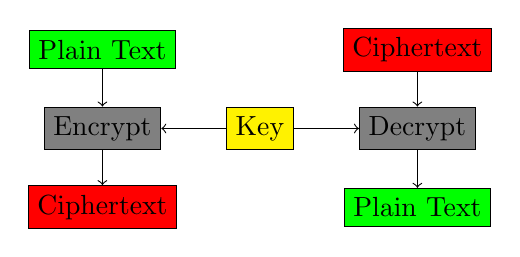
\begin{tikzpicture}[node distance=2cm]
	\node[draw, fill=green] (plainOne) at (0,2) {Plain Text};
	\node[draw, fill=gray] (encrypt) at (0,1) {Encrypt};
	\node[draw, fill=red] (cipherOne) at (0,0) {Ciphertext};
	\node[draw, fill=yellow] (key) at (2,1) {Key};
	\node[draw, fill=red] (cipherTwo) at (4,2) {Ciphertext};
	\node[draw, fill=gray] (decrypt) at (4,1) {Decrypt};
	\node[draw, fill=green] (plainTwo) at (4,0) {Plain Text};
	
	\draw[->,draw=black] (plainOne) to (encrypt);
	\draw[->,draw=black] (encrypt) to (cipherOne);
	\draw[->,draw=black] (key) to (encrypt);
	\draw[->,draw=black] (key) to (decrypt);
	\draw[->,draw=black] (cipherTwo) to (decrypt);
	\draw[->,draw=black] (decrypt) to (plainTwo);
	\end{tikzpicture}
	
}
\frame{\frametitle{Asymmmetric Encryption}
	Public key and private key pair \newline
	Public key is used to encrypt a message\newline
	Private key is used to decrypt a message\newline
	Creating the key tends to be computationally expensive\newline
	
	\center
	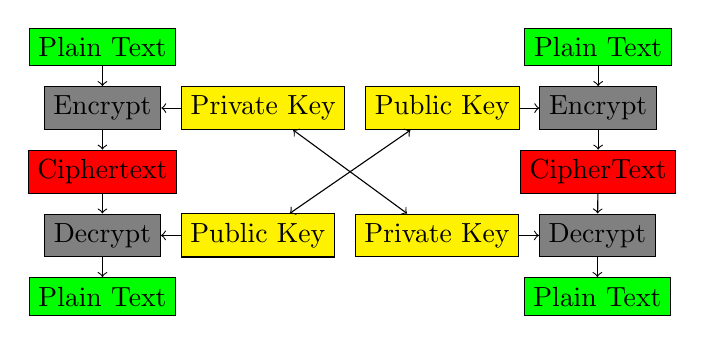
\begin{tikzpicture}[node distance=.25cm]
		\node[draw, fill=green] (plainOne) {Plain Text};
		\node[draw, fill=gray, below = of plainOne] (encryptpriv) {Encrypt};
		\node[draw, fill=red, below = of encryptpriv] (cipherOne) {Ciphertext};
		\node[draw, fill=yellow, right = of encryptpriv] (keypriv) {Private Key};
		\node[draw, fill=gray, below = of cipherOne] (decryptpub)  {Decrypt};
		\node[draw, fill=green, below = of decryptpub] (plainTwo) {Plain Text};		
		\node[draw, fill=yellow, right = of decryptpub] (keypub)  {Public Key};
	
		\node[draw, fill=yellow, right = of keypriv] (keypubtwo) {Public Key};
		\node[draw, fill=yellow, right = of keypub] (keyprivtwo) {Private Key};
		\node[draw, fill=gray, right = of keypubtwo] (encryptpub) {Encrypt};
		\node[draw, fill=gray, right = of keyprivtwo] (decryptpriv) {Decrypt};
		\node[draw, fill=green, below = of decryptpriv] (plainFour) {Plain Text};
		\node[draw, fill=green, above = of encryptpub] (plainThree) {Plain Text};
		\node[draw, fill=red, below = of encryptpub] (cipherThree) {CipherText};
		
		
		\draw[->,draw=black] (plainOne) to (encryptpriv);
		\draw[->,draw=black] (encryptpriv) to (cipherOne);
		\draw[->,draw=black] (keypriv) to (encryptpriv);
		\draw[->,draw=black] (cipherOne) to (decryptpub);
		\draw[->,draw=black] (keypub) to (decryptpub);
		\draw[->,draw=black] (decryptpub) to (plainTwo);
		
		\draw[->,draw=black] (plainThree) to (encryptpub);
		\draw[->,draw=black] (encryptpub) to (cipherThree);
		\draw[->,draw=black] (keypubtwo) to (encryptpub);
		\draw[->,draw=black] (cipherThree) to (decryptpriv);
		\draw[->,draw=black] (keyprivtwo) to (decryptpriv);
		\draw[->,draw=black] (decryptpriv) to (plainFour);
		
		\draw[<->, draw=black] (keypub) to (keypubtwo);
		\draw[<->, draw=black] (keypriv) to (keyprivtwo);
		
	\end{tikzpicture}
}


\frame{\frametitle{Hashing}
	
	
}



\frame{\frametitle{Hybrid Encryption}
	Uses ideas from symmetric and asymmetric encryption methods \newline
	An asymmetric cryptosystem is used for key encapsulation and an symmetric system is used for data encapsulation\newline
	
		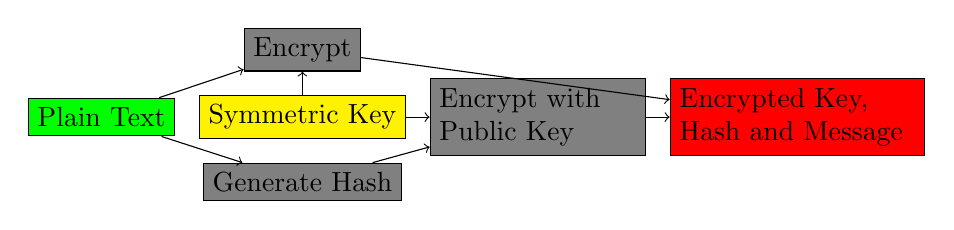
\begin{tikzpicture}[node distance=.3cm]
		\node[draw, fill=gray] (encrypt) {Encrypt};
		\node[draw, fill=yellow, below = of encrypt] (symkey) {Symmetric Key};
		\node[draw, fill=gray, below = of symkey] (hash) {Generate Hash};
		\node[draw, fill=green, left = of symkey] (plaintext) {Plain Text};
		\node[draw, fill=gray, right = of symkey, text width = 2.5cm] (encryptpub) {Encrypt with Public Key};
		\node[draw, fill=red, right = of encryptpub, text width = 3cm] (asymencrypt) {Encrypted Key, Hash and Message};
		
		
		\draw[->,draw=black] (plaintext) to (encrypt);
		\draw[->,draw=black] (plaintext) to (hash);
		\draw[->,draw=black] (hash) to (encryptpub);
		\draw[->,draw=black] (symkey) to (encrypt);
		\draw[->,draw=black] (symkey) to (encryptpub);
		\draw[->,draw=black] (encrypt) to (asymencrypt);
		\draw[->,draw=black] (encryptpub) to (asymencrypt);
		
		\end{tikzpicture}
}

\frame{\frametitle{Cyclic Groups}
	
	
}


\frame{\frametitle{RSA Cryptosystem}
	
}

\frame{\frametitle{ElGamal Cryptosystem}
	
}

\frame{\frametitle{Elliptic Curve}
	
}

\frame{\frametitle{Conclusion}
	
}

\frame{\frametitle{Demo!}
	
}


\frame{\frametitle{References}
	http://caislab.kaist.ac.kr/lecture/2010/spring/cs548/basic/B02.pdf
	
	
}
\end{document}
